\section{Databricks vs. EMR Presto reference results}\label{referenceResults}

This section presents the reference results obtained by executing the full TPC-DS benchmark at the 1 TB scale factor employing the hardware and software configuration described in Section \ref{experimentalSetup}.

\subsection{Data loading}\label{referenceResultsDataLoading}

The TPC-DS Toolkit includes a data generator that produces raw text files that can be subsequently processed by a data framework to generate data files and accompanying metadata suitable for efficient query processing. The metadata is stored in a Hive-compatible metastore and the data in column-storage format files.

The raw text files generated for the 1 TB scale factor chosen for the reference results actually add up to 910.7 GB. The files were generated with 4 parallel streams, thus for some tables the data comprises 4 separate files, which are stored in the same directory. The format is raw text with the octal character \textbackslash 001 used as the column separator, which is the default in both Databricks and EMR Presto. It should be noted, however, that (unlike Databricks) EMR Presto does not allow in its supported syntax to employ an alternative character as separator. All of these files are stored in their respective directories within a common AWS S3 bucket.

The raw text files are used to create external tables by means of custom CREATE TABLE statements for Databricks and EMR Presto. We use these tables only for accessing data, not query processing. Additional CREATE TABLE statements are used to create another set of external tables employing a column-storage format, these meant for query processing. The data from the raw text external tables is fed to the external column-storage tables by means of INSERT INTO statements. The column-storage table files are also stored in S3. The format used for Databricks is Parquet with SNAPPY compression; the files add up to 297.5 GB, yielding a compression ratio of 3.26. Although Presto also supports the Parquet format, experiments showed that better results are achieved with the ORC format, using SNAPPY compression as well. The ORC files for Presto add up to 246.1 GB, resulting in a compression ratio of 3.94.

It is important to remark that for the reference results we present in this section, the tables were not explicitly analyzed to yield table and column statistics for optimization. The generation of table-level or basic statistics is different for each system. EMR Presto generates them by default with the execution of the INSERT INTO statements, which does not occur with Databricks. Thus for the query processing experiments, unless stated otherwise, EMR Presto has basic table statistics available while Databricks does not. In addition, neither system produces by default column-level statistics. Although Presto has the capability to compute column statistics, our EMR Presto configuration employs AWS Glue for table metadata, which does not support column statistics. On the other hand, Databricks does support them and we explore their effects in Section \ref{databricksWithStatistics}. Finally, we remark that we did not consider custom data partitioning in any of our experiments.

The behavior of the systems in regards to the data loading process as described above is summarized in Figure 18.

\begin{figure}
   \begin{center}
   \scalebox{0.65}{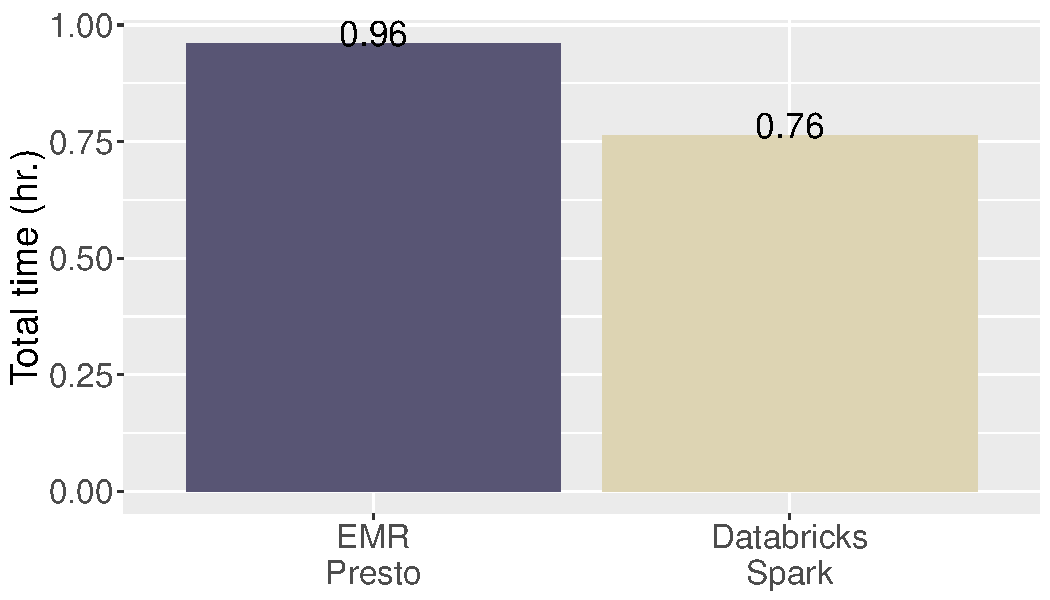
\includegraphics[width=7.0in]{imgs/referenceResults/load_totalHrTimeBarChart.pdf}}
   \end{center}
   \caption{Reference results Data Loading Test total time.}
   \label{fig:referenceResultsDataLoading}
\end{figure}

\subsection{Individual query execution (Power Test)}\label{referenceResultsPowerTest}

